\section{Effects of Real Grounds}
\subsection{Relative Permitivity and Conductivity in Boulder, Colorado}
Using material published by the American Radio Relay League, the estimated
ground conductivity in Boulder, Colorado was found to be 15 mS/m \cite{antbook}, which
is consistent with the description of rocky soil and mountainous terrain. A
more specific region was selected as the effective ground conductivity varied
noticeably across the state from 2-15 mS/m. The relative permitivity
$\epsilon_r$ for the region that describes Boulder varies between 12-14. As a
result, $\epsilon_r$ for Boulder was assumed to be 13. 

\subsubsection{Effects on Gain}
After modeling the ground plane in FEKO, a change in the Gain was observed as
shown in Figure~\ref{fig:gpol}. Here, it can be seen that the point where the
transmission power is greatest is directed upwards
such that $\theta_{Ground}<\theta_{Ideal}$.

\begin{figure}[h!]
  \centering
  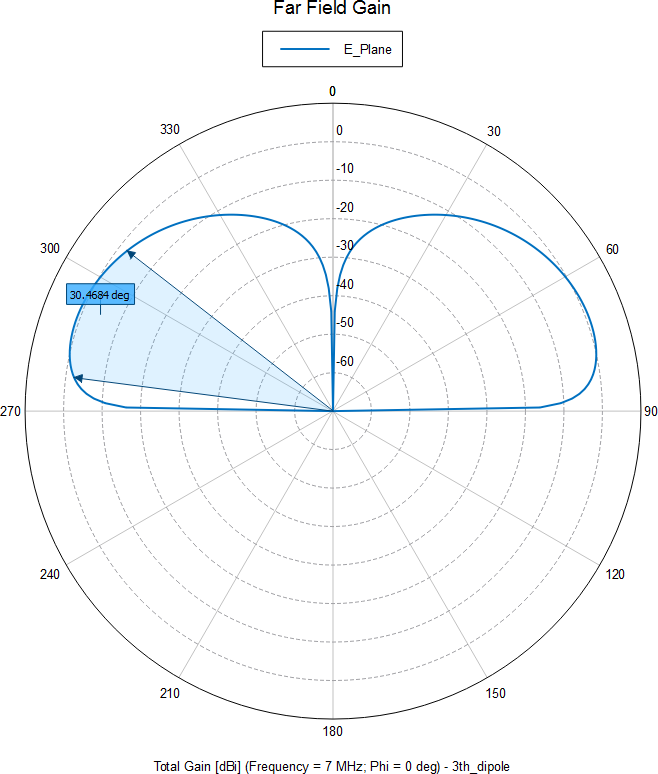
\includegraphics[width=0.40\textwidth]{./img/gndgain.png}
  \caption{$\vec{E}$ field plot and 3dB beamwidth considering ground effects} 
  \label{fig:gpol}
\end{figure}

\subsubsection{Effects on Efficiency}
The change in Efficiency was the most significant change after applying the
ground.
Using the Equation (\ref{eq:eff}), the efficiency was found:
\begin{align}
  \eta_A&=P_{Rad}(1-L_M)^2\label{eq:eff}
\end{align}
Where $\eta_A$ is the radiation efficiency, $P_{Rad}$ is the total
radiated power and $L_M$ is the mismatch loss. All of these quantities can be
calculated using FEKO. At the 7MHz point, the efficiency with the ground was
found to be 80.38\%, in contrast to the 92.3\% efficiency in free space.
\subsubsection{Effects on Impedance}
After adding in the ground, the antenna's resonance changed from 7 MHz to about
6.9 MHz, as seen in Figure~\ref{fig:gimp}.
\begin{figure}[h!]
  \centering
  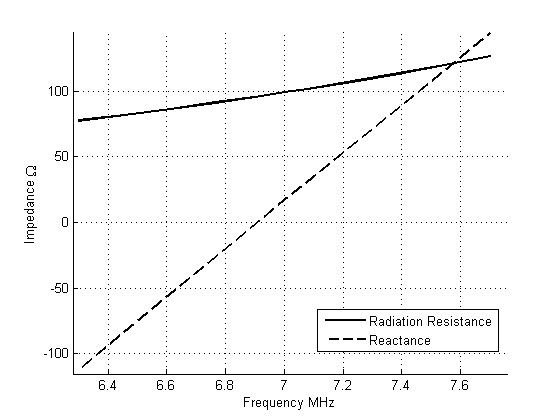
\includegraphics[width=0.45\textwidth]{./img/gimpedance.png}
  \caption{Impedance versus frequency accounding for ground effects}
  \label{fig:gimp}
\end{figure}

\subsubsection{Effects on Radiation Pattern}
Having a ground plane under the antenna is akin to having a somewhat reflective
surface under a tubular flourescent lamp; RF energy that is reflected from the
surface of the ground interferes with the waves that would otherwise travel
straight, causing an overall change in the shape of the $\vec{E}$ field shown
in Figure~\ref{fig:gpol}. The 3D pattern is shown in Figure~\ref{fig:g3d}.
Interestingly, this makes the antenna somewhat safer to be around as, instead
of having the full force of the transceiver be directly across from the
antenna, most of the power is instead directed upwards.

\begin{figure}[h!]
  \centering
  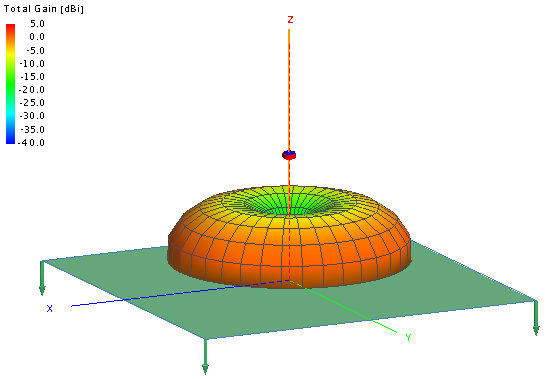
\includegraphics[width=0.45\textwidth]{./img/g3dgain.png}
  \caption{$\vec{E}$ field plot considering a ground and 3dB beamwidth}
  \label{fig:g3d}
\end{figure}
